\documentclass[9pt]{beamer}
\usepackage[sfdefault]{roboto}
\usepackage{styles/fluxmacros}
\usefolder{styles}
\usetheme[style=asphalt]{flux}
\usepackage{xcolor}
\usepackage{color}
\usepackage{amsmath}
\usepackage{amssymb}
\usepackage{graphicx}
\usepackage{latexsym}
\usepackage[T1]{fontenc}
\usepackage[utf8]{inputenc}
\usepackage{wrapfig}
\usepackage{siunitx}
\usepackage{times}
\usepackage{tikz}
\usepackage{verbatim}
\usepackage{multimedia}
\usepackage{hyperref}
\usepackage{thumbpdf}
\usepackage{%
    pgf,%
    pgfarrows,%
    pgfnodes,%
    pgfautomata,%
    pgfheaps,%
    pgfshade%
}
\usepackage{url}
\usepackage{empheq}
\usepackage{fancybox}
\usepackage{esint}
\usepackage{lipsum}
\usepackage{listings}
\usepackage{mathptmx}
\usepackage{helvet}
\usepackage{tikz}%
\usepackage{circuitikz}
\usepackage{csvsimple}
\usepackage{pgfplots}
\usepackage{multimedia}
\usepackage{proba}
\usepackage[absolute,overlay]{textpos}
\usepackage{bibunits}
\usepackage{tcolorbox}
\usepackage{qrcode}
%\usepackage[texcoord,%
%            grid,%
%            gridunit=mm,%
%            gridcolor=red!60,%
%            subgridcolor=black!60%
%            ]{eso-pic}
\usepackage{enumerate}
\usepackage[makeroom]{cancel}
\usepackage{epstopdf}
\usepackage{booktabs}
\usepackage{calc}
\usepackage{enumitem}
\usepackage{algorithmic,algorithm}
\setbeamercovered{transparent}
% Informations

\epstopdfsetup{outdir=./}
\mode<presentation>
{
    \useinnertheme{progressbar}
}
%\setbeamertemplate{items}[ball]
%~~~~~~~~~~~~~~~~~~~~~~~~~~~~~~~~~~~~~~~~~~~~-~~~~~~~~~~~~~~~~~~~~~~~~~~~~~~~~~~
%~~~~~~~~~~~~~~~~~~~~~~~~~~~~~~~~~~~~~~~~~~~~~-~~~~~~~~~~~~~~~~~~~~~~~~~~~~~~~~~
% Informations
\defaultbibliography{main}
%
\title{\Huge{Maximum likelihood estimation}\\
    \Huge{
        \textbf{
            for a stochastic SEIR system}
    }
}
\subtitle{%
        \textbf{
            \textcolor{gray}{
                 an application of the Grisanov's%
            }
       }
    \\    
    \textbf{    
        \textcolor{gray}{
            Theorem for the likelihood ratio
        }
    }    
    \\
    \normalsize{March 28, 2022}
}
%
\author{
    \normalsize{%
        CONACYT-UNISON-UNAM: FDV, FBL, SDIV
    }
}
%
\titlegraphic{assets/logo-unison.png}
%~~~~~~~~~~~~~~~~~~~~~~~~~~~~~~~~~~~~~~~~~~~~~~~~~~~~~~~~~~~~~~~~~~~~~~~~~~~~~~
%%%%%%%%%%%%%%%%%%%%%%%%%%%%%%%%%%%%%%%%%%%%%%%%%%%%%%%%%%%%%%%%%%%%%%%%%%%%%%%%

\def\Q#1#2{\frac{\partial #1}{\partial #2}}
\usetikzlibrary{arrows,shapes}
\pgfplotsset{compat=1.14}
\pgfplotstableread[col sep = comma]{noise/Images/Introduction/gbm.csv}\mydata
\epstopdfsetup{outdir=./}
%%%%%%%%%%%%%%%%%%%%%%%%%%%%%%%%%%%%%%%%%%%%%%%%%%%%%%%%%%%%%%%%%%%%%%%%%%%%%%%%
%-----------------------------ExtrasDeTercerPresentacion
%--------------------------------Fancyboxes-------------------------------------
\definecolor{myblue}{rgb}{.8, .8, 1}
\definecolor{azure(colorwheel)}{rgb}{0.0, 0.5, 1.0}
\definecolor{shadecolor}{cmyk}{0,0,0.41,0}
\newcommand*\mybluebox[1]{%
    \colorbox{myblue}{\hspace{1em}#1\hspace{1em}}
}
\newcommand*\myyellowbox[1]{%
    \colorbox{darkyellow}{\hspace{1em}#1\hspace{1em}}
}
%--------------------------------------------------------------------------
\definecolor{shadecolor}{cmyk}{0,0,0.41,0}
\definecolor{light-blue}{cmyk}{0.25,0,0,0}
\newsavebox{\mysaveboxM} % M for math
\newsavebox{\mysaveboxT} % T for text
\newcommand*\Garybox[2][Example]{%
    \sbox{\mysaveboxM}{#2}%
        \sbox{\mysaveboxT}{\fcolorbox{black}{light-blue}{#1}}%
            \sbox{\mysaveboxM}{%
    \parbox[b][\ht\mysaveboxM+.5\ht\mysaveboxT+.5\dp\mysaveboxT][b]{%
        \wd\mysaveboxM}{#2}%
    }%
    \sbox{\mysaveboxM}{%
        \fcolorbox{black}{shadecolor}{%
        \makebox[\linewidth-10em]{\usebox{\mysaveboxM}}%
        }%
    }%
    \usebox{\mysaveboxM}%
    \makebox[0pt][r]{%
        \makebox[\wd\mysaveboxM][c]{%
            \raisebox{\ht\mysaveboxM-0.5\ht\mysaveboxT
            +0.5\dp\mysaveboxT-0.5\fboxrule}{\usebox{\mysaveboxT}}%
        }%
    }%
}
\newcommand\Fontvi{\fontsize{7}{7.2}\selectfont}
%%%%%%%%%%%%%%%%%%%%%%%%%%%%%%%%%%%%%%%%%%%%
\definecolor{kugreen}{RGB}{50,93,61}
\definecolor{kugreenlys}{RGB}{132,158,139}
\definecolor{kugreenlyslys}{RGB}{173,190,177}
\definecolor{kugreenlyslyslys}{RGB}{214,223,216}
\definecolor{greenArea}{RGB}{124,252,124}
\definecolor{hellmagenta}{rgb}{1,0.75,0.9}
\definecolor{hellcyan}{rgb}{0.75,1,0.9}
\definecolor{hellgelb}{rgb}{1,1,0.8}
\definecolor{colKeys}{rgb}{0,0,1}
\definecolor{colIdentifier}{rgb}{0,0,0}
\definecolor{colComments}{rgb}{1,0,0}
\definecolor{colString}{rgb}{0,0.5,0}
\definecolor{darkyellow}{rgb}{1,0.9,0}
\setbeamercovered{transparent}
\lstset{%
    language=[AlLaTeX]TEX,%
    float=hbp,%
    basicstyle=\ttfamily\small, %\usepackage{cir}
    identifierstyle=\color{colIdentifier}, %
    keywordstyle=\color{colKeys}, %
    stringstyle=\color{colString}, %
    commentstyle=\color{colComments}, %
    columns=flexible, %
    tabsize=3, %
    frame=single, %
    extendedchars=true, %
    showspaces=false, %
    showstringspaces=false, %
    numbers=left, %
    numberstyle=\tiny, %
    breaklines=true, %
    backgroundcolor=\color{hellgelb}, %
    breakautoindent=true, %
    captionpos=b,%
    xleftmargin=18pt,%
    xrightmargin=\fboxsep%
}
\pgfplotsset{
    left segments/.code={\pgfmathsetmacro\leftsegments{#1}},
    left segments=3,
    left/.style args={#1:#2}{
        ybar interval,
        domain=#1:#2,
        samples=\leftsegments+1,
        x filter/.code=\pgfmathparse{\pgfmathresult}
       }
}
\DeclareMathOperator{\sign}{sgn}
\newcommand{\innerprod}[2]{\left\langle#1, #2\right\rangle}
\newcommand\bound{10} % bound number of points on each side of N
\newcommand\labelnum[3][]{
    \begin{scope}[font=\footnotesize,x=.3cm,#1]
      \foreach \mypt in {0,#2,...,\bound}{
        \draw(\mypt,0)circle[radius=2pt];
        \draw(-\mypt,0)circle[radius=2pt];
      }
      \draw(-\bound-5,0)--(\bound+5,0) node[pos=0, left]{$t$};
      \node(start)[at={(-\bound-4,0)},label=below:{$t_0=0$}]{$[$};
      \node(end)[at={(\bound+4,0)},label=below:{$T=Nh$}]{$]$};
      \node[%
          at={($(start)!.319!(end)$)},
          label=below:{
               $\underbrace{}_{h}$
            }%
            ]{\vphantom{$[$}};
      \node[at={($(start)!.57!(end)$)},label=below:{$t_{n+1}$}]{\vphantom{$[$}};
      \filldraw(0,0)circle[radius=2pt];
      \node[at={(-\bound-2,0)},above]{$\cdots$};
      \node[at={(\bound+2,0)},above]{$\cdots$};
      \node[at={(0,0)},above=5pt]{#3};
    \end{scope}
}
\usepackage{remreset}
\makeatletter
\@removefromreset{subsection}{section}
\makeatother
\definecolor{greenstrong}{rgb}{0.58,0.77,0.29}
\definecolor{redstrong}{rgb}{0.81,0.22,0.23}
\definecolor{fglisting}{gray}{0.3}
\definecolor{bglisting}{gray}{1}
\definecolor{fgshell}{gray}{1}
\definecolor{bgshell}{gray}{0.1}
\definecolor{bgshelllight}{gray}{0.8}
\definecolor{cadmiumorange}{rgb}{0.93, 0.53, 0.18}
\definecolor{capri}{rgb}{0.0, 0.75, 1.0}
%
\setcounter{subsection}{1}
\newcommand{\hl}[1]{\textbf{\textcolor{greenstrong}{#1}}}
\newcommand{\hb}[1]{\textbf{\textcolor{azure(colorwheel)}{#1}}}
\newcommand{\hlErr}[1]{\textcolor{redstrong}{\texttt{#1}}}
\newcommand{\hlOk}[1]{\textcolor{green}{\texttt{#1}}}
\newcommand{\hlInv}[1]{\colorbox{bgshell}{\textcolor{fgshell}{\texttt{#1}}}}
\newcommand{\unhl}[1]{\textcolor{gray}{#1}}
\newcommand{\clda}[0]{$\textcolor{blue}{\lambda}$}
\newcommand{\carr}[0]{$\textcolor{purple}{\rightarrow}$}
\newcommand{\cbind}[0]{\textbf{\texttt{$>\!\!>\!\!=$}}}
\newcommand{\codedots}[0]{\textcolor{mid-gray}{...}}

%
\tcbuselibrary{skins, breakable}
\newtcolorbox{greenbox}[1]{%
        colback = green!5!white,
        colframe = green!55!black,
        fonttitle = \bfseries,
        title = #1 %
    }
\newtcolorbox{bluebox}[1]{%
        colback = blue!5!white,
        colframe = blue!55!black,
        fonttitle = \bfseries,
        title = #1
    }
%
\newtcolorbox{graybox}[1]{%
        colback = gray!5!white,
        colframe = gray!55!black,
        fonttitle = \bfseries,
        title = #1
    }
%
\newtcolorbox{yellowbox}[1]{%
        colback = yellow!5!white,
        colframe = yellow!55!black,
        fonttitle = \bfseries,
        title = #1
    }

\newcolumntype{P}[1]{>{\centering\arraybackslash}p{#1}}
\begin{document}
    \titlepage
         \section*{Introduction}
    \part{Modeling with Noise}
        \section{Modeling with SDEs}
             \defaultbibliography{noise/noise.bib}
\defaultbibliographystyle{abbrv}
\begin{frame}[plain]%{Why SDE?}{UQ}
        \begin{empheq}[box={\Garybox[UQ]}]{equation*}
            ODE + noise = Better \  Model
        \end{empheq}
%
%   \begin{overlayarea}{\textwidth}{.8\textheight}
%        \begin{columns}
%            \column{.5\textwidth}
%            \only<2-3>{
%                \begin{exampleblock}{Population growth}
%                    $$
%                        \frac{dN}{dt}=a(t)N(t) \qquad N_0=N(0)=cte.
%                    $$
%                \end{exampleblock}
%            }
%            \only<4-6>{
%            \begin{exampleblock}{Electric Circuits}
%                \begin{align*}
%                   &L\cdot Q''(t)+
%                    R\cdot Q'(t)+
%                    \frac{1}{C}\cdot Q(t)
%                        =F(t)
%                    \\
%                   &Q(0)=Q_0\\
%                   &Q'(0)=I_0
%                \end{align*}
%            \end{exampleblock}
%        }
%        \column{.58\textwidth}
%        \only<3>{
%            \begin{empheq}[box=\shadowbox*]{equation*}
%                a(t)=r(t)+"noise"
%            \end{empheq}
%        }
%        \only<5-6>{
%            %\includegraphics[width=\textwidth]{./images/CircuitRLC.png}
%            \begin{circuitikz}[american voltages]
%                \draw (0,0)
%                to[sV,v=$F(t)$] (0,2) % The voltage source
%                to[R=$R$, i^>=$i(t)$] (2,2) % The resistor
%                to[L=$L$] (4,2)
%                to[C=$C$] (4,0)--(0,0) ;
%            \end{circuitikz}
%        }
%        \only<6>{
%            \begin{textblock*}{55 mm}(75mm,60mm)
%                \begin{empheq}[box=\shadowbox*]{equation*}
%                    F(t)=G(t)+"noise"
%                \end{empheq}
%            \end{textblock*}
%        }
%        \end{columns}
%    \end{overlayarea}
\end{frame}
% %%%%%%%%%%%%%%%%%%%%%%%%%%%%%%%%%%%%%%%%%%%%%%%%%%%%%%%%%%%%%%%%%%%%%%%%%%%%%%%%%%
\begin{frame}
    \frametitle{To fix ideas}
    \begin{empheq}[box=\Garybox]{align*}
        dN(t) = aN(t)dt
    \end{empheq}
    \begin{overlayarea}{\textwidth}{.3\textheight}
        \begin{columns}
            \column{.5\textwidth}
                \only<2->{
                    \begin{block}{Perturb in $[t, t+dt)$}
                        \only<3->{
                            $$
                              a dt
                              \rightsquigarrow
                              a dt + \sigma dB(t)
                            $$
                        }
                    \end{block}
               }
            \column{.5\textwidth}
        \only<4->{
            \begin{exampleblock}{Get a SDE}
              $$
               dN(t) = aN(t)dt + \sigma N(t) dB(t)
              $$
            \end{exampleblock}
        }
        \end{columns}
    \end{overlayarea}
    \begin{overlayarea}{\textwidth}{.7\textheight}
        \centering
            \resizebox{0.45\textwidth}{!}{%
            \only<5>{
                \begin{tikzpicture}
                    \begin{axis}[%
                     line width=1.0pt,
                     mark size=1.0pt,
                     x label style={at={
                        (axis description cs:0.5,-0.1)
                        },anchor=north},
                     y label style={at={
                        (axis description cs:0.0,.5)},anchor=south
                     },
                     xlabel={$t$},
                     ylabel={$N(t)$}
                    ]%
                         \addplot[color=blue]%
                         table [%
                           x index = {0},
                           y index = {1} %
                       ]{\mydata};
                       \addplot[domain=0:5, samples=100]{1.5*exp(x)};
                    \end{axis}
                \end{tikzpicture}
         }
        }
    \end{overlayarea}
\end{frame}
% %%%%%%%%%%%%%%%%%%%%%%%%%%%%%%%%%%%%%%%%%%%%%%%%%%%%%%%%%%%%%%%%%%%%%%%%%%%%%
 \begin{frame}[plain,noframenumbering]
    \frametitle{Some Important applications}
    \begin{columns}
        \column{.3\textwidth}
         \begin{overlayarea}{\textwidth}{.3\textheight}
             \begin{itemize}%[<+-|alert@+>]
                 %
                 \item
                     Finance
                 \item
                     Physics
                 \item
                     Chemistry
                 \item
                     Biology
                 \item
                     Epidemiology
             \end{itemize}
        \end{overlayarea}
        \column{.7\textwidth}
        \begin{overlayarea}{\textwidth}{.5\textheight}
            \begin{exampleblock}{

                     \only<1>{Henston}
                     \only<2>{Langevin}
                     \only<3>{Brusselator}
                     \only<4>{Lotka Volterra}
                     \only<5>{SIR}
                 }
                 \only<1>{
                     \begin{align*}
                        dS_t &= \mu S_t dt + \sqrt{V_t}S_t
                            \left(
                                \sqrt{1- \rho^2}dW^{(1)}_t
                                + \rho dW^{(2)}
                            \right)
                        \\
                        dV_t &=
                            \kappa (\lambda - V_t)dt +
                            \theta \sqrt{V_t} dW^{(2)}_t
                     \end{align*}
                 }
                 \only<2>{
                     \begin{equation*}
                        dX_t = -(\nabla U) (X_t) dt + \sqrt{2\epsilon}dW_t
                     \end{equation*}
                 }
                \only<3>{
                    \begin{align*}
                         dX_t =&
                             \left[
                                 \delta
                                 -(\alpha + 1) X_t +
                                 Y_t X_t^2
                             \right] dt
                             + g_1(X_t) dW_t^{(1)}
                        \\
                         dY_t =&
                             \left[
                                 \alpha X_t +
                                 Y_t X_t^2
                             \right] dt
                             + g_2(X_t) dW_t^{(2)}
                        \\
                    \end{align*}
                 }
                \only<4>{
                    \begin{align*}
                        dX_t &=
                            (\lambda X_t - k X_t Y_t ) dt +\sigma X_t dW_t
                        \\
                        dY_t &= (k X_t Y_t -mY_t) dt
                    \end{align*}
                }
                \only<5>{
                    \begin{align*}
                        dS_t & = (-\alpha S_t I_t - \delta S_t + \delta) dt
                            - \beta S_t I_t dW_t
                        \\
                        dI_t & = (\alpha S_t I_t - (\gamma + \delta) I_t) dt
                            + \beta S_t I_t dW_t
                        \\
                        dR_t & =
                            (\gamma I_t  - \delta R_t) dt
                    \end{align*}
                }
             \end{exampleblock}
         \end{overlayarea}
    \end{columns}
    %
    \only<1-4>{
        \begin{bibunit}[apalike]
            \nocite{Hutzenthaler2015}
            \putbib
        \end{bibunit}
    }
    \only<5>{
    \begin{bibunit}[apalike]
        \nocite{Tornatore2005}
        \putbib
    \end{bibunit}
    }
 \end{frame}

        \section{Perturbation of parameters}
             \begin{frame}
    \frametitle{Why noise?}
    \begin{textblock*}{37mm}(3mm, 10mm)
        \begin{block}{Environmental effects}
            \begin{itemize}
                \item \textcolor<2-3>{orange}{Extinction}
                \item \textcolor<4>{orange}{Outbreaks}
            \end{itemize}
        \end{block}
    \end{textblock*}
    \begin{textblock*}{75mm}(50mm, 10mm)
        \begin{alertblock}{%
            \only<2>{%
                    Environmental Brownian noise suppresses
                    explosions.
                    %
            }%
            \only<3>{%
                    Noise color induces extinction
            }%
            \only<4>{%
                $\mathcal{R}_0$: Endemic g.a.e. $\to$ periodic oscillations
            }%
        }%Block titles
            \only<2>{
                    \begin{bibunit}[apalike]
                        \nocite*{Mao2002}
                        \putbib
                    \end{bibunit}
            }
            \only<3>{
                \begin{bibunit}[apalike]
                    \nocite*{Ripa1996}
                    \putbib
                \end{bibunit}
            }
            \only<4>{
                \begin{bibunit}[apalike]
                    \nocite*{Allen2013}
                    \putbib
                \end{bibunit}
            }
        \end{alertblock}
    \end{textblock*}
\end{frame}
             \begin{frame}
    \frametitle{Alternativas}
    \begin{textblock*}{37mm}(3mm, 50mm)
        \begin{block}{Environmental effects}
            \begin{itemize}
                \item Extinction
                \item Outbreaks
            \end{itemize}
        \end{block}
    \end{textblock*}
%%%%%%%%%%%%%%%%%%%%%%%%%%%%%%%%%%%%%%%%%%%%%%%%%%%%%%%%%%%%%%%%%%%%%%%%%%%%%%%
    \begin{textblock*}{37mm}(3mm, 15mm)
        \begin{block}{In Biology}
            \begin{itemize}
                \item<1> \textcolor<1>{orange}{\textbf{DTMC, CTMC}}
                \item<2-3>\textcolor<2-3>{orange}{
                    \textbf<2-3>{%
                        Stochastic perturbation of parameters
                    }
                }
                \item<4> \textcolor<4>{orange}{Mean reverting processes}
            \end{itemize}
        \end{block}
    \end{textblock*}
%%%%%%%
    \begin{textblock*}{65mm}(55mm, 35mm)
        \begin{alertblock}{%
                \only<1>{%
                    $\mathbf{DTMC}+\mathbf{CTMC}+\mathbf{ME} \to SDE$%
                }%
                \only<2>{%
                    $\varphi dt \rightsquigarrow \varphi dt + \sigma dB_t$%
                }%
                \only<3>{%
                    $\varphi dt \rightsquigarrow \varphi dt + F(x)dB_t$%
                }%
                \only<4>{%
                    $d \varphi_t = (\varphi_e -\varphi_t)dt + \sigma_\varphi
                    dBt$ %
                }%
            }%Block titles
            \only<1>{
                \begin{bibunit}[apalike]
                    \nocite{Allen2017}
                    \putbib
            \end{bibunit}
            }
            \only<2>{
                \begin{bibunit}[apalike]
                    \nocite{Gray2011}
                    \putbib
            \end{bibunit}
            }
            \only<3>{
                \begin{bibunit}[apalike]
                    \nocite{Schurz2015}
                    \putbib
                \end{bibunit}
            }
            \only<4>{
                \begin{bibunit}[apalike]
                    \nocite{Allen2016}
                    \putbib
                \end{bibunit}
            }
        \end{alertblock}
    \end{textblock*}
\end{frame}

%             \begin{frame}
    \frametitle{Formulation of SDE: $DTMC \to CTMC + ME \to SDE$}
    \begin{textblock*}{50mm}(5mm, 10mm)
        To fix ideas, we recall the
        deterministic philosophy to
        formulate ODEs
        \begin{enumerate}[label=(\roman*)]
            \item<2-> 
                We study a process in an small interval of
                time $\Delta t$
            \item<3->
                Describe the resulting information in $\Delta t$
            \item<4->
                Letting $\Delta t \to 0$ gives an ODE
        \end{enumerate}
    \end{textblock*}
% %
     \only<5>{
         \begin{textblock*}{50mm}(70mm, 10mm)
            \begin{exampleblock}{Newton's Cooling Law}
                $
                    T_A(t + \Delta t) - T_A(t) = 
                        \alpha (T_B - T_A(t)) \Delta t
                $
                $   \displaystyle
                    \frac{T_A(t + \Delta t) - T_A(t)}{\Delta t}
                    = \alpha (T_B - T_A(t)) 
                $
                Letting $\Delta t \to 0$
                $$   \displaystyle
                    \frac{dT_A(t)}{dt}
                    = \alpha (T_B - T_A(t))
                $$
            \end{exampleblock}
        \end{textblock*}
        \begin{textblock*}{60mm}(75mm, 47.5mm)
            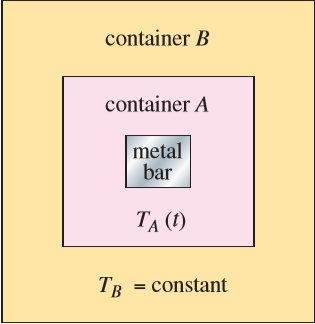
\includegraphics[width=0.7\linewidth]{noise/Images/Assets/newton_cooling_law}
        \end{textblock*}
    }
\end{frame}
% %
\begin{frame}
    \frametitle{Formulation of SDE: $DTMC \to CTMC + ME \to SDE$}
%
        \begin{textblock*}{60mm}(5mm, 15mm)
            A stochastic analogy.
            \begin{enumerate}[label=(\roman*)]
                \item<2->
                    Formulate a discrete stochastic
                    model for the dynamical system
                    understudy, which describe changes
                    in a small time interva $\Delta t$
                \item<3->
                    Compute the expected value and
                    covariance for the difference in a short
                    time $\Delta t$
                \item<4->
                    Letting $\Delta t \to 0$, 
                    he above information
                    leads to the CTMC
                \item<5->
                    Thus, we infer the SDE from the
                    similarities in the forward-backward-Kolmogorov equation 
                    between the
                    discrete and Continuous Markov
                    Chain
            \end{enumerate}
        \end{textblock*}
\end{frame}
% %
\begin{frame}% frame 00
    \frametitle{Example: Formulation of a stochastic SIS model}
    \begin{textblock*}{50mm}(5mm, 10mm)
    Consider the deterministic SI model:
        \begin{align*}
            \frac{dS}{dt} &= -\frac{\beta}{N} S I + (b +\gamma) I
                \\
            \frac{dI}{dt} &= \frac{\beta}{N} S I - (b +\gamma) I
                \\
            N &= S(t)+ I(t)
        \end{align*}
        Where $N$ is constant and  $S(t) = N - I(t)$.
    \end{textblock*}
    \only<2->{
        \begin{textblock*}{50 mm}(60mm, 10mm)
            \begin{empheq}[box=\shadowbox]{align*}
                \mathcal{R}_0 &= 
                    \frac{\beta}{b + \gamma}
                    \\
                \mathcal{R}_0 & \leq 1
                \\
                & \Rightarrow
                    \lim_{t \to \infty} (S(t),N(t)) = (N, 0)
                \\
                \mathcal{R}_0 & > 1
                \\
                & \Rightarrow
                    \lim_{t \to \infty} (S(t),N(t)) = (S^*, I^*)
            \end{empheq}
        \end{textblock*}
    }
\end{frame}
% %
% %
\begin{frame}{Example: Formulation of a stochastic SIS model}
    \begin{textblock*}{55mm}(5mm, 10mm)
        Consider the process $\{\mathcal{I}_t\}_{t=0} ^ \infty$ with 
        time discrete and space of states $\{0,1,\cdots, N \}$.
        \begin{enumerate}[label=(H-(\arabic*)]
            \item <2->
                \begin{align*}
                    p_i(t) &:= \probX{\mathcal{I}(t) = i}
                    \\
                    i &= 0,1,2\dots, N
                    \\
                    t &= 0, \Delta t, 2 \Delta t, \cdots,
                \end{align*}
            \item <3->
                Markov property
                $$
                    \probCX{I_{t + \Delta t}}{  I_0, I_{\Delta t}, \cdots, I_t}
                    =\probCX{I_{t + \Delta t} }{I_t}
                $$
            \item <4->
                The unique transitions with positive 
                probability
                \begin{align*}
                    & p_{ji}(t + \Delta t)
                    = 
                    \probCX{I_{t + \Delta t} = j}{I_t = i}
                    \\
                    &\text{are}
                    \\
                    & i \to i+1, \ i \to i-1,  \ i \to i
                \end{align*}
        \end{enumerate}
    \end{textblock*}
    \only<5->{
        \begin{textblock*}{50mm}(55mm, 10mm)
            \begin{equation*}
                p_{ji}(\Delta t):=
                    \begin{cases}
                        \frac{\beta i (N - i)}{N} \Delta t, 
                            & j = i + 1
                        \\
                        (b + \gamma) i \Delta t, 
                            & j = i - 1
                        \\
                        1 - 
                        \left[
                            \frac{\beta i (N - i)}{N} +
                            (b + \gamma) i
                        \right]
                        \Delta t, 
                            & j=i,
                        \\
                        0 & \text{otherwise}
                \end{cases}
            \end{equation*}
            where $\Delta t$ is sufficiently small s.t.
            $$
                \max_{i \in \{ 1, \dots, N \}}
                \{
                    [b(i) + d(i)] \Delta t
                \}
                \leq 1
            $$
        \end{textblock*}
    }
    \only<6>{
        \begin{textblock*}{50mm}(65mm, 60mm)
            \begin{center}
                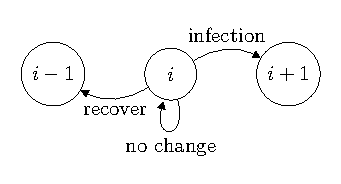
\includegraphics[width=\linewidth]{noise/Images/Assets/chain.pdf}
            \end{center}
        \end{textblock*} 
     }
\end{frame}
%%%%%%%%%%%%%%%%%%%%%%%%%%%%%%%%%%%%%%%%%%%%%%%%%%%%%%%%%%%%%%%%%%%%%%%%%%%%%%%%
\begin{frame}{Example: Formulation of a stochastic SIS model}
    \only<2->{
    \begin{textblock*}{55mm}(5mm, 10mm)
        Letting
        \begin{align*}
            b(i) &:= \frac{\beta i (N - i)}{N} \Delta t
            \\
            d(i) &:= (b + \gamma) i \Delta t
        \end{align*}
    \end{textblock*}
    }
    \only<3->{
        \begin{textblock*}{90mm}(45mm, 8mm)
            \begin{empheq}[box={\Garybox[FKE]}]{align*}
                p_i(t + \Delta t) &=
                    p_{i-1}(t) b(i - 1) \Delta t 
                    \\
                    & + p_{i+1}(t) d(i + 1) \Delta t
                    \\
                    & + p_i(t) (1 -[b(i) + d(i)] \Delta t)
            \end{empheq}
        \end{textblock*}
    }
    \only<4->{
    \begin{textblock*}{140mm}(-3mm, 35mm)
        \hspace{5em} Thus $P(\Delta t) = $
        \begin{equation*}
            \begin{pmatrix}
            1   & d(1) \Delta t & 0 & \cdots    & 0 & 0
            \\
            0   & 1 - (b+d)(1) \Delta t & d(2)  \Delta t   & \cdots    & 0   & 
            0 
            \\
            0   & b(1) \Delta t  & 1 - (b+d)(2) \Delta t   & \cdots    & 0 & 0
            \\
            0 & 0 & b(2) \Delta t & \cdots    & 0 & 0
            \\
            \vdots & \vdots & \vdots & \ddots & \vdots & \vdots
            \\
            0 & 0 & 0 & \cdots & d (N - 1) \Delta t  & 0
            \\
            0 & 0 & 0 & \cdots & 1- (b+d) (N - 1) \Delta t  & d(N) \Delta t
            \\
            0 & 0 & 0 & \cdots & d (N - 1) \Delta t  &  1 - d(N) \Delta t 
            \end{pmatrix}
        \end{equation*}
        \begin{textblock*}{100mm}(10mm, 80mm)
            $$
                p(t + \Delta t) = P(\Delta t) p(t) = P^{n+1}(\Delta t) p(0), 
                \qquad t =n \Delta t
            $$
        \end{textblock*}
    \end{textblock*}
    }
\end{frame}
% %
% %
\begin{frame}{Expected Value of the SIS-DTMC}
    \begin{textblock*}{80mm}(15mm,6mm)
        \begin{align*}
            \only<2->{
                \E(I_{t + \Delta t}) 
                &=  
                    \sum_{i = 0} ^ N
                        i p_i(t + \Delta t)
            }
            \\
            \only<3->{
                &=
                        \sum_{i = 0} ^ N
                            i p_{i - 1} (t) b(i - 1) \Delta t
                    + \sum_{i = 0} ^ {N-1}
                            i p_{i + 1} (t) d(i + 1) \Delta t
                \\       
                    &+ 
                        \sum_{i=0}^N i p_i(t) \Delta t
                        - \sum_{i=0}^N i p_i(t) b(i) \Delta t
                        - \sum_{i=0}^N i p_i(t) d(i) \Delta t
            }
            \\
            \only<4>{
                \E(I_{t+ \Delta t}) 
                    &= 
                    \E(I_t) 
                        + \sum_{i = 1} ^ N
                            p_{i-1} (t)
                            \frac{\beta (i-1)(N - [i -1])}{N} \Delta t
                \\
                        &-
                            \sum_{i = 0} ^ {N - 1}
                            p_{i + 1} (t) (b + \gamma) (i+1) \Delta t
                \\
                    &=
                    \E(I_t) + [\beta - (b + \gamma )] \Delta t \E(I_t)
                    -\frac{\beta}{N} \Delta t 
                    \underbrace{\E(I_t ^ 2)}_{\geq \E ^2(I_t)}
            }
        \end{align*}
    \end{textblock*}
%
\end{frame}
% %%%%%%%%%%%%%%%%%%%%%%%%%%%%%%%%%%%%%%%%%%%%%%%%%%%%%%%%%%%%%%%%%%%%%%%%%%%%%%%%
\begin{frame}{Expected Value of the SIS-DTMC}
    \begin{textblock*}{60mm}(20mm, 25mm)
       \begin{equation*}
            \frac{\E(I_{t + \Delta t}) - \E(I_t)}{\Delta t}
                \leq
                    [\beta  - (b + \gamma)] \E (I_t)
                    - \frac{\beta}{N} \E^2 (I_t)
        \end{equation*}
        %
        \only<2->{
            \begin{align*}
                \frac{d \E(I_{t})}{dt}
                    & \leq
                        [\beta  - (b + \gamma)] \E (I_t)
                        - \frac{\beta}{N} \E ^ 2 (I_t)
                \\
                    & = \frac{\beta}{N} [N - \E(I_t)] \E (I_t)
                        - (b + \gamma) \E (I_t)
            \end{align*}
        }
        \only<3->{
            \begin{empheq}[box=\shadowbox]{equation*}
                \frac{d \E(I_{t})}{dt}
                \leq
                \frac{\beta}{N} \E(S_t) \E (I_t)
                    - (b + \gamma) \E (I_t)
            \end{empheq}
        }
    \end{textblock*}
\end{frame}
%%%%%%%%%%%%%%%%%%%%%%%%%%%%%%%%%%%%%%%%%%%%%%%%%%%%%%%%%%%%%%%%%%%%%%%%%%%%%%%%
\begin{frame}{Example: Formulation of a stochastic SIS model}
    \begin{textblock*}{55mm}(5mm, 10mm)
        \begin{empheq}[box=\shadowbox]{align*}
            N &= 100, \ \Delta t = 0.01, \ \beta = 1, 
            \\
            b &= 0.25 \ \gamma = 0.25 
        \end{empheq}
    \end{textblock*}
%
    \begin{textblock*}{100mm}(5mm, 20mm)
        \begin{center}
            \includegraphics[width=\linewidth]{%
                noise/Images/Assets/random_walk_SIS%
            }
        \end{center}
    \end{textblock*}
%
    \begin{textblock*}{20mm}(105mm, 20mm)
        \begin{empheq}[box=\fbox]{align*}
            \mathcal{R}_0 &= 2,  
             \\
            \bar{I} &= 50
        \end{empheq}
    \end{textblock*}
\end{frame}
% %
%
%        \section*{Continuous Time Markov Chains (CTMC}
%             \begin{frame}{Formulating a SIS-CTMC }
    \begin{textblock*}{60mm}(20mm, 25mm)
        Let 
        $
                \{ I_t\}_{t \geq 0}, p_i(t) = \probX{I_t = i}.
        $
        \only<2->{
            Thus, the Markov property becomes in
            \begin{align*}
                \probCX{ I_{t_{n + 1}}}{I_{t_0}, \cdots, I_{t_n} }
                    &=
                    \probCX{ I_{t_{n + 1}}}{I_{t_n}}
                    \\
                    \text{for all } &
                    t_0 < t_1 < \cdots < t_n 
            \end{align*}
        }
    \end{textblock*}
    \only<3>{
        \begin{textblock*}{90mm}(20mm, 50mm)
            \begin{align*}
                &p_{ji}(\Delta t):=
                    \begin{cases}
                        \frac{\beta i (N - i)}{N} \Delta t 
                            + o(\Delta t),     
                            & j = i + 1
                        \\
                        (b + \gamma) i \Delta t 
                            + o(\Delta t),
                            &   j = i - 1
                        \\
                        1 - \left [
                                \frac{\beta i (N - i)}{N} +
                                (b + \gamma) i %                
                            \right] \Delta t
                            + o(\Delta t) , 
                            & j=i
                        \\
                        o(\Delta t) & \text{otherwise}
                    \end{cases}
                \\
                & \lim_{t\to \infty}
                    \frac{o(\Delta t)}{\Delta t}
                    = 0
            \end{align*}
        \end{textblock*}
    }
\end{frame}
 %%%%%%%%%%%%%%%%%%%%%%%%%%%%%%%%%%%%%%%%%%%%%%%%%%%%%%%%%%%
\begin{frame}{}
    \begin{textblock*}{90mm}(10mm, 5mm)
        Using the notation for birth and death
        processes, we have
        \begin{equation*}
            p_{ij}(\Delta t):=
                \begin{cases}
                    b(i) \Delta t + o(\Delta t),     
                        & j = i + 1
                    \\
                    d(i) \Delta t + o(\Delta t), 
                        &   j = i - 1
                    \\
                    1 - \left [
                            b(i) + d(i) %                
                        \right] \Delta t
                        + o(\Delta t), 
                        & j=i
                    \\
                    0 & \text{otherwise}.
                \end{cases}
        \end{equation*}
    \end{textblock*}
    \only<2->{    
        \begin{textblock*}{90mm}(10mm, 30mm)       
            $\probX{I_0 = i_0} = 1$,
            \begin{align*}
                p_i(t + \Delta t)
                    =&
                        p_{i - 1} (t) b(i -1) \Delta t
                        \\
                        & + 
                            p_{i + 1} (t) d(i + 1) \Delta t
                        \\
                        & +
                            p_{i} (t)[1 - (b(i) + d(i))] \Delta t
                        + o(\Delta t)
                \\
                i &= 1, 2, \dots, N
            \end{align*}
        \end{textblock*}
    }
    \only<3->{
        \begin{textblock*}{90mm}(10mm, 60mm)              
            Thus
            \begin{align*}
                \frac{p_i (t - \Delta t) - p_i (t) }{\Delta t}
                = & 
                p_{i - 1} (t) b(i-1)
                    +
                    p_{i + 1} (t) d(i+1)  
                \\
                    &-
                    p_i [b(i) + d (i)] 
                    +o(\Delta t)
                \\
                & i = 1,2,\cdots, N.
            \end{align*}
        \end{textblock*}
    }
    \end{frame}
%%%%%%%%%%%%%%%%%%%%%%%%%%%%%%%%%%%%%%%%%%%%%%%%%%%%%%%%%%%%%%%%
\begin{frame}{}
    \begin{textblock*}{60mm}(10mm, 10mm)       
        Hence, letting $\Delta t \to 0$,  we obtain
        \begin{align*}
            \frac{dp_i(t)}{dt}
            = & 
            p_{i - 1} (t) b(i-1)
                +
                p_{i + 1} (t) d(i+1)  
            \\
                &-
                p_i [b(i) + d (i)] 
            \\
                & i = 1,2,\cdots, N.
        \end{align*}
    \end{textblock*}
    \only<2->{        
        \begin{textblock*}{60mm}(65mm, 10mm)       
            \begin{empheq}[box=\fbox]{align*}
                FKE:  &\frac{dp}{dt} = Q p
                \\
                p(t) & = (p_0(t), \dots, p_N(t)) ^ {\top}
            \end{empheq}
        \end{textblock*}
    }
    \only<3->{
        \begin{textblock*}{90mm}(10mm, 30mm)
            \begin{equation*}
                Q = 
                \begin{pmatrix}
                    0   & d(1)  & 0 & \dots     & 0
                    \\
                    0   & -[b(1) + d(1)]    & d(2)  & \dots     & 0
                    \\
                    0   & b(1)  & -[b(2) + d(2)]    & \dots     & 0     
                    \\
                    0   & 0     & b(2)  & \dots     & 0
                    \\
                    \vdots  & \vdots    & \vdots    & \ddots    & \vdots
                    \\
                    0   & 0     & 0     & \dots     & d(N)
                    \\
                    0   & 0     & 0     & \dots     & -d(N)    
                \end{pmatrix}
            \end{equation*}
            \only<4->{
                Results that
                $$
                    \lim_{t \to \infty}
                        p(t) = (1, 0, \dots, 0)^{\top}
                $$
                and
                $$
                    Q = \lim_{\Delta t \to 0}
                        \frac{P(\Delta t) - I}{\Delta t}
                $$
            }
        \end{textblock*}
    }
\end{frame}
%%%%%%%%%%%%%%%%%%%%%%%%%%%%%%%%%%%%%%%%%%%%%%%%%%%%%%%%%%%%%%%%%%%%%%%%%%%
\begin{frame}{Expected value of the SIS-CTMC}
    \begin{textblock*}{50mm}(10mm, 20mm)
        Consider the m.g.f    
        \begin{align*}
            M(\theta, t)&:= 
            \E [\exp( \theta I_t)]
            \\
            &= \sum_{i = 0} ^ N
                p_i(t) \exp( i \theta)
        \end{align*}
    \end{textblock*}   
    \only<2->{
        \begin{textblock*}{60mm}(65mm, 20mm)
            Results that
            $$
                \E[I_t ^ k] =
                    \frac{\partial ^ k M}{\partial \theta ^ k}
                    \big |_{\theta = 0},
                    \quad k=1,2 , \dots, 
            $$
            
            
        \end{textblock*}
    }
    \only<3>{
        \begin{textblock*}{120mm}(15mm, 50mm)
            Now we deduce a differential equation
            for the moments of our sis-CTMC.
        \end{textblock*}
    }
\end{frame}
%%%%%%%%%%%%%%%%%%%%%%%%%%%%%%%%%%%%%%%%%%%%%%%%%%%%%%%%%%%%%%%%%%%%%%%%%%%
\begin{frame}{}
    \begin{textblock*}{100mm}(10mm, 10mm)
        \begin{align*}
            \frac{\partial M}{\partial t}
                =&
                    \sum_{i = 0} ^ N 
                        \frac{d p_i}{dt}
                        \exp(i \theta)
                \\
                \only<2>{
                    \text{from r.h.s of  FKE} &
                    \\
                        = &
                        \exp(\theta) 
                            \sum_{i = 0} ^N 
                                p_{i - 1} \exp[(i - 1) \theta] b(i-1)
                    \\
                        & +
                        \exp(- \theta)
                            \sum_{i = 0} ^N 
                                p_{i + 1} \exp[(i + 1) \theta] d(i + 1)
                    \\
                        & -
                        \sum_{i = 0} ^ N
                            p_i \exp(i \theta) (b(i) + d(i))
                }
        \end{align*}
    \end{textblock*}
\end{frame}
%%%%%%%%%%%%%%%%%%%%%%%%%%%%%%%%%%%%%%%%%%%%%%%%%%%%%%%%%%%%%%%%%%%%%%%%%%%
\begin{frame}{}
    Substituting definition of $b, d$
    we obtain
    \begin{align*}
        \frac{\partial M}{\partial t} 
        =&
            \beta(exp(\theta) -1) 
                \sum_{i = 1}^N i 
                    p_i \exp(i \theta)
        \\    
        &+ 
            (b + \gamma)(\exp(- \theta) -1) 
                \sum_{i=1}^N 
                    i p_i \exp(i\theta)
        \\
        & -
            \frac{\beta}{N} (\exp(\theta) - 1)
                \sum_{i=1}^N
                    i ^ 2 p_i \exp(i \theta)
        \\
        \only<2>{
            = &
                [
                    \beta(exp(\theta) -1)
                    (b + \gamma)(\exp(- \theta) -1)
                ] \frac{\partial M}{ \partial \theta}
            \\
            & -
                \frac{\beta}{N} (\exp(\theta) - 1)
                \frac{\partial ^ 2 M}{\partial \theta^2}
        }
    \end{align*}
\end{frame}
%%%%%%%%%%%%%%%%%%%%%%%%%%%%%%%%%%%%%%%%%%%%%%%%%%%%%%%%%%%%
\begin{frame}{}
    \begin{bibunit}[apalike]
        Following \cite{Bailey1964} we can deduce from the above equation
        \begin{equation*}
        \frac{d \E (I_t)}{dt} =
            [\beta - (b + \gamma)] \E(I_t)
            - \frac{\beta}{N}
                \E(I_t ^2).
        \end{equation*}
        Then we conclude as in the SIS-DTMC.
        \putbib
    \end{bibunit}
\end{frame}
%%%%%%%%%%%%%%%%%%%%%%%%%%%%%%%%%%%%%%%%%%%%%%%%%%%%%%%%%%%%%  
\begin{frame}{}
    Using the Guillespie algorithm
         \includegraphics[width=\textwidth, keepaspectratio]%
         {noise/Images/Assets/random_walk_SIS-CTMC.png}
\end{frame}

%        \section*{SDEs}
%             %%%%%%%%%%%%%%%%%%%%%%%%%%%%%%%%%%%%%%%%%%%%%%%%%%%%%%%%%%%%%%%%%
\begin{frame}{Formuling a SIS-SDE}
    \begin{overlayarea}{\textwidth}{\textheight} 
        Now, consider $\{I_t\}_{t \geq 0}$. 
        \only<2->{
            For fixed time $t$
            $I_t$ is a r.v, assume that  $I_t$
            has a probability density 
            function $p(x,t)$.
        }
        \only<3->{
            That is,
            \begin{equation*}
                \probX{a \leq I_t \leq b}
                    = \int_{a}^{b}
                    p(x,t) dx.
            \end{equation*}
        }
        %     
        \only<4->{
            $I_t$ is Markovian.
        }
    %  
        \only<5->{
            \begin{align*}
                &\probCX{I_{t_{n}} \leq y}{I_{t_0}, \cdots, I_{t_{n-1}} }
                    =
                        \probCX{ I_{t_{n}} \leq }{I_{t_{n-1}}}
                    \\
                        \text{for all } &
                        0 \leq t_0 < t_1 < \cdots < t_n
            \end{align*}
        }
        
        \only<6->{
            Denote the transition p.d.f as
            \begin{align*} 
                & p(y, t + \Delta t; x ,t)
                \\
                & y = I_{t + \Delta t},
                \quad x =I_t
        \end{align*}
        }
    \end{overlayarea}
\end{frame}
%%%%%%%%%%%%%%%%%%%%%%%%%%%%%%%%%%%%%%%%%%%%%%%%%%%%%%%%%%%%%%%%%%%%%%%%%%%%
\begin{frame}{}
     Set $\Delta i = 1$, then
    \begin{overlayarea}{\textwidth}{\textheight}
         \begin{align*}
            \only<2->{
                \frac{d p_i}{dt} 
                    =&
                    p_{i -1} b(i-1) + p_{i + 1} d(i + 1)
                    - p_i [ b(i) + d(i)]
            }
            \\
            \only<3->{
                &=
                - \frac{
                    p_{i + 1}[d(i + 1) - d(i + 1)]
                    - 
                    p_{i - 1}[d(i -1) - d(i - 1)]
                }{2 \Delta i}           
            \\
                & +
                \frac{1}{2}
                \frac{
                    p_{i + 1}[d(i + 1) + d(i + 1)]
                    -
                    2 p_i[b(i) + d(i)]
                    +
                    p_{i - 1}[d(i -1) + d(i - 1)]}{
                        (\Delta_i) ^ 2
                    }
            }
        \end{align*}       
        \only<4->{
            Let $i = x$, $\Delta i = \Delta x$ and $pi(t) = p(x,t)$.
            Thus, letting  $\Delta x \to 0$, we obtain the FKE
        }
        \only<5->{
            \begin{align*} 
                \frac{\partial p(x,t)}{\partial t}
                    =&
                        \frac{\partial}{\partial x} \{   
                                [b(x) - d(x)] p(x,t)
                            \}
                    +
                        \frac{1}{2}
                            \frac{\partial ^ 2}{\partial t ^ 2} \{
                                b(x)  + d(x) p(x,t) 
                            \}
                    \\
                    =&
                        \frac{\partial}{\partial x}
                        \left \{
                            \left [
                                \frac{\beta}{N}
                                x (N - x)
                                - (b + \gamma) x
                            \right]
                            p(x,t)
                        \right \}
                    \\    
                    &+
                        \frac{1}{2}
                        \frac{\partial ^ 2}{\partial x ^ 2}
                        \left \{
                            \left [
                                \frac{\beta}{N}
                                    x (N -x) + (\beta + \gamma) x 
                            \right ] p(x, t)
                        \right \}
            \end{align*}
        }
    \end{overlayarea}
 \end{frame}
%%%%%%%%%%%%%%%%%%%%%%%%%%%%%%%%%%%%%%%%%%%%%%%%%%%%%%%%%%%%%%%%%%    
\begin{frame}{}
    Using the SIS-CTMC probablity transition kernel 
    \begin{overlayarea}{\textwidth}{\textheight}
        \begin{align*}
            &p_{ji}(\Delta t):=
                \begin{cases}
                    \frac{\beta i (N - i)}{N} \Delta t 
                        + o(\Delta t),     
                        & j = i + 1
                    \\
                    (b + \gamma) i \Delta t 
                        + o(\Delta t),
                        &   j = i - 1
                    \\
                    1 - \left [
                            \frac{\beta i (N - i)}{N} +
                            (b + \gamma) i %                
                        \right] \Delta t
                        + o(\Delta t) , 
                        & j=i
                    \\
                    o(\Delta t) & \text{otherwise}.
                \end{cases}
        \end{align*}
        \only<2->{
            If increment $\Delta t$ follows a 
            exponential distribution  and is suficiently small.
            Results that increment 
            $$
                \Delta I = I_{t + \Delta t} - I_t
            $$  
            has normal distribuition, with following expectation and variance.
            \\
        }
        \only<3->{
            Fix time $t$ s.t  $I_t = i$
            \begin{align*}
                \E{\Delta I}
                    =&
                        b(I_t) \Delta t - d(I_t) \Delta t + o(\Delta t)
                    \\
                    &=
                        \underbrace{
                            [b(I)_t - d(I_t)]
                        }_{:=\mu(I_t)} + o(\Delta t) 
            \end{align*}
        }
    \end{overlayarea}
\end{frame}    
%%%%%%%%%%%%%%%%%%%%%%%%%%%%%%%%%%%%%%%%%%%%%%%%%%%%%%%%%%%%%%%%%%%%%%%%%%%%
\begin{frame}{}
    Thus
    \begin{overlayarea}{\textwidth}{\textheight}
        \only<2->{
            \begin{align*}
                \VarX{\Delta I_t}
                    &=
                        \EX{\Delta I_t ^ 2} - [\EX{\Delta I_t}] ^ 2
                    \\
                    & = 
                        \underbrace{
                            [b(I_t)  + d(I_t) ]
                        }_{:=\sigma^2(I_t)}
                            \Delta t + o(\Delta t).
            \end{align*} 
        }
        \only<3->{
            Since 
            $
                \Delta I_t \sim \mathcal{N}
                    (
                    \mu(I_t) \Delta t, 
                    \sigma ^ 2 (I_t) \Delta t
                )
            $,
            we see that 
        }
        \only<4->{
            \begin{align*}
                I_{t+\Delta t} 
                    &= 
                        I_t + \Delta I_t
                \\
                    &\approx
                        I_t + \mu(I_t)\Delta t 
                        + \sigma(I_t) \sqrt{\Delta t} \eta
                \\
                    & \eta \sim \mathcal{N}(0,1)
            \end{align*}
            The Euler-Maruyama's recurrence equation.
        }
    \end{overlayarea}
\end{frame}
%%%%%%%%%%%%%%%%%%%%%%%%%%%%%%%%%%%%%%%%%%%%%%%%%
\begin{frame}{}
    \begin{overlayarea}{\textwidth}{.8\textheight}
        Further, becouse under this setting, the Euler-Maruyama converge.   
        \only<2->{
            Letting $\Delta t \to 0$, we deduce our SIS-SDE:
            \begin{equation*}
                dI_t = \mu(I_t) + \sigma(I_t) dW_t.
            \end{equation*}
        }
        \only<3->{
            Sustituting, the notation for birth and death processes
            \begin{equation*}
                dI_t =
                    \frac{\beta}{N} I_t(N - I_t)
                    - (b + \gamma) I_t
                    +
                    \sqrt{
                        \frac{\beta}{N} 
                            I_t (N - I_t)
                            +
                            (b + \gamma)I_t
                    }
                    dW_t.
            \end{equation*}
        }
    \end{overlayarea}
\end{frame}
%%%%%%%%%%%%%%%%%%%%%%%%%%%%%%%%%%%%%%%%%%%%%%%%%%%%%%%
\begin{frame}{}  
    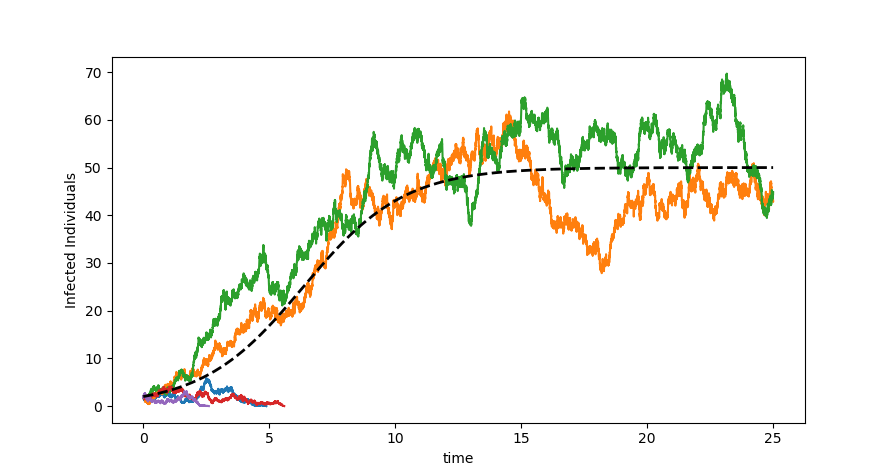
\includegraphics[width=\textwidth,keepaspectratio=true]{%
        noise/Images/Assets/random_walk_SIS-SDE.png%
    }
\end{frame}

        \begin{frame}
            \frametitle{Table of contents}
            \tableofcontents
        \end{frame}
        \section{Parameter estimation of SEIR-Covid-19 model based on a SDE}
	        \begin{frame}{CDMX Covid-19 data}
    \begin{figure}[htb]
        \centering
        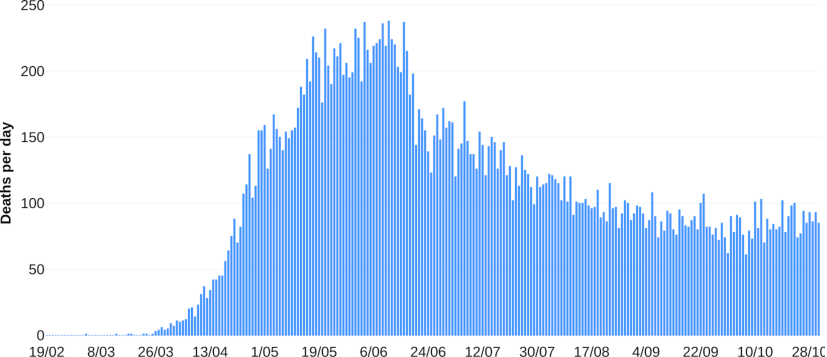
\includegraphics[width=0.8\textwidth, keepaspectratio]{%
            sto_mle_covid19/Figures/CDMX_dta.png%
        }
        \caption{%
            CDMX data
        }
        \label{fig:data_CDMX_fitting}
    \end{figure}
\end{frame}


\begin{frame}{An application to the estimation of parameters}
    \begin{Huge}
        \begin{description}
            \item[Example:]
                Estimation of the infection rates
                $\beta_s$, $\beta_a$, and ratio of asymptomatic cases $p$.
            \item[Argument:]
                Noise could improve the
                uncertainty quantification.
        \end{description}
    \end{Huge}
    \footnote{
        Work in progress. 
        \\ Somited in IJCM.
        Fernado Baltazar (UNAM-CU) and Francisco Delgado
        (CONACYT-UNAM-OAXACA)}
\end{frame}
%------------------------------------------------------------
\begin{frame}{MCMC with a deterministic SEIRS structure}
    \begin{textblock*}{120mm}(0mm, 10mm)
        \only<1->{        
            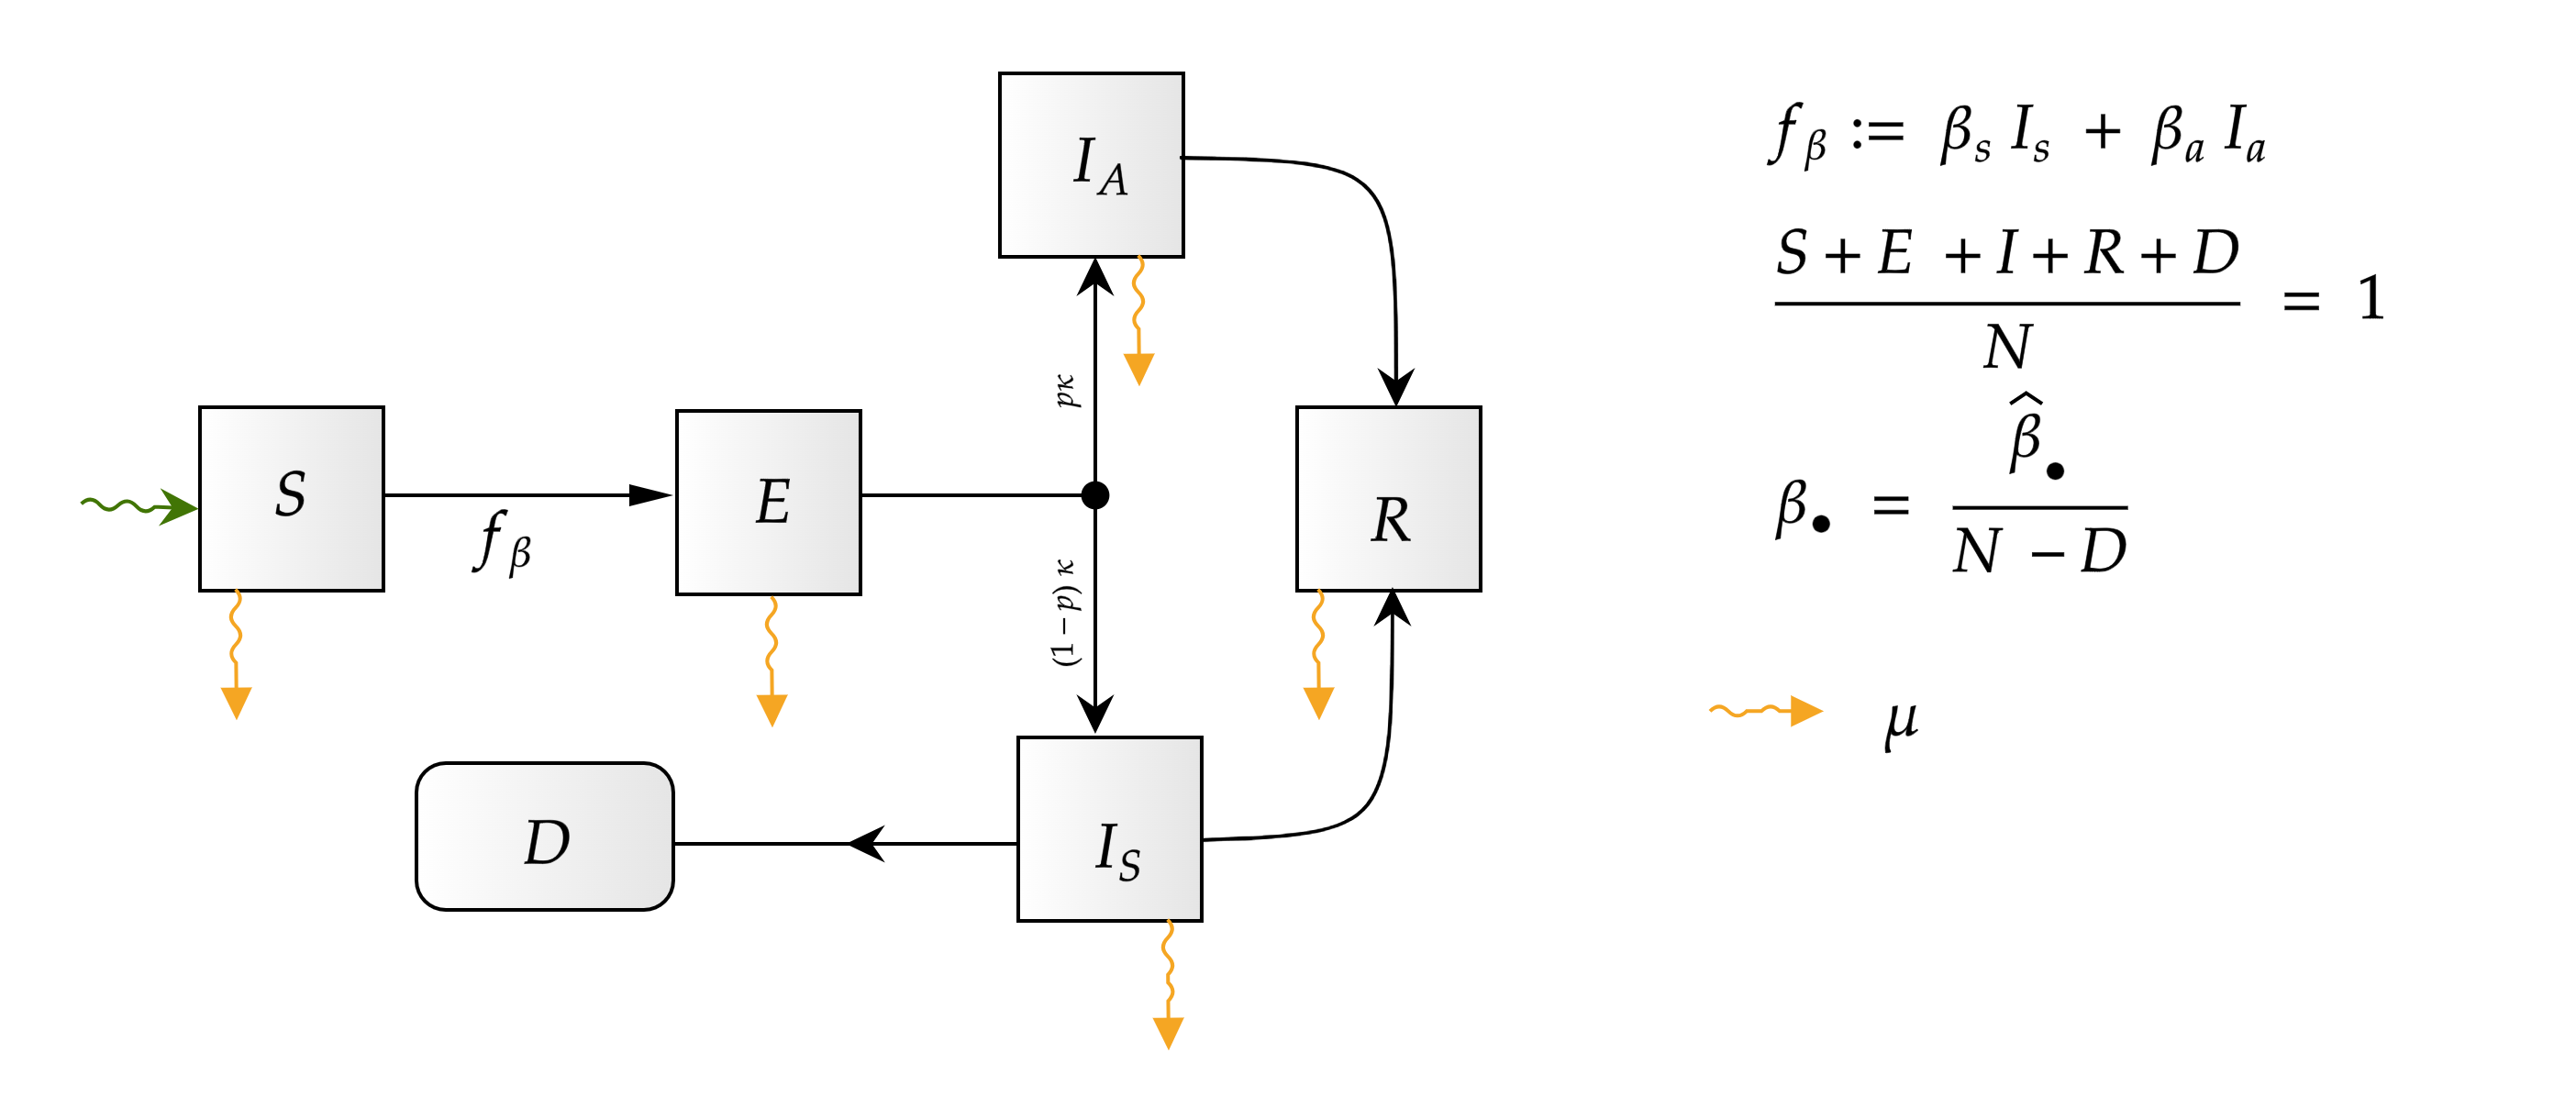
\includegraphics[width=\textwidth]{assets/stoSEIR_diagram.png} 
        }
    \end{textblock*}    
%    
%%    
    \begin{textblock*}{60mm}(0mm, 50mm)
	    \only<2->{
	        \begin{equation*}
	            \label{eqn:base_dynamics}
	            \begin{aligned}
	                S'  &=
	                    \mu +\gamma R
	                    - \left(\mu  + f_{\beta} \right)  S
	                \\
	                 E' & =  f_{\beta}S
	                     - (\kappa E + \mu E
	                     )
	                \\
	                {I_a}' &=
	                    p \kappa E
	                    - \big(\alpha_a + \mu \big)I_a
	                \\
	                 {I_s}' &=
	                    (1 - p) \kappa E
	                    - (\alpha_s +\mu)  I_s
	                \\
	                {R}' &=
	                    \alpha_a I_a + \alpha_s (1 - \theta)I_s -
	                    (\mu + \gamma) R
	                \\
	                D' &= \theta \alpha_s I_s.
	            \end{aligned}
	        \end{equation*}
	     }
    \end{textblock*}
%%    
    \begin{textblock*}{60mm}(65mm, 55mm)
	    \only<3>{
	        \begin{equation*}
	            \label{eqn:base_dynamics_counter}
	            \begin{aligned}
	                Y_t & \sim
	                    \mathrm{Poisson}(\lambda_t)
	                \\
	                    \lambda_t =& \int_0 ^ t (1-p) \kappa E
	                \\
	                    p & \sim
	                    \mathrm{Uniform}(0.3, 08)
	                \\
	                    \kappa & \sim
	                    \mathrm{Gamma}(10, 50)
	                \\
	                    \beta_a, \beta_s & \sim\mathcal{N}(0.5,0.1)    
	            \end{aligned}
	        \end{equation*}
	    }
    \end{textblock*}
\end{frame}
%%%%%%%%%%%%%%%%%%%%%%%%%%%%%%%%%%%%%%%%%%%%%%%%%%%%%%%%%%%%%%%%%%%%%%%%%%%%%%%%
\begin{frame}{Overfiting example}
    \begin{figure}[htb]
        \centering
        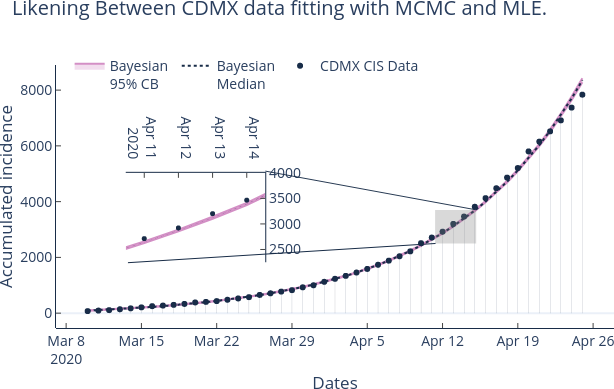
\includegraphics[width=0.8\textwidth, keepaspectratio]{%
            sto_mle_covid19/Figures/MCMC_CDMXDataFitting.png%
        }
        \caption{%
            MCMC Fit of diary new cases of Mexico city
            during exponential growth. See
            \url{https://plotly.com/~sauld/53/} for an electronic
            version.
        }
        \label{fig:data_CDMX_fitting}
    \end{figure}
\end{frame}
            \begin{frame}{Stochastic perturbation}
    \begin{textblock*}{60mm}(10mm, 15mm)
        Perturbing the above deterministic base by Brownian Motion
    \end{textblock*}
%
    \begin{textblock*}{100mm}(20mm, 30mm)
        \begin{graybox}{
                $\mu dt\rightsquigarrow \mu dt + \sigma dW(t)$ gives
                our SDE SEIR-Covid-19
        }
            \begin{equation*}
                \begin{aligned}
                    d {S}(t)  =&
                    \big[\mu - \mu S(t) - f_{\beta} S(t)
                    +\gamma R(t)  \big] dt 
                    + \color{orange}{
                        \sigma \big(1- S(t)\big) dW(t)
                    }
                    \\
                    d {E}(t) =& \big[  f_{\beta} S(t)
                    - \kappa  E(t) - \mu E(t) \big] dt  
                    - \color{orange}{
                        \sigma E(t) dW(t)
                    }
                    \\
                    d {I_a}(t) =& \big[
                        p \kappa E(t)
                        -   (\alpha_a +\mu) I_a(t)  \big] dt  
                        - \color{orange}{
                            \sigma I_a(t) dW(t)
                        }
                    \\
                    d {I_s}(t) =& \big[
                        (1 - p) \kappa E (t)
                        - (\alpha_s +\mu)  I_s(t) \big] dt   
                        - \color{orange}{
                            \sigma I_s(t) dW(t)
                        }
                    \\
                    d {R}(t) =&
                        \big[
                        \alpha_a I_a(t) +
                        \alpha_s I_s(t) - (\mu + \gamma) R(t)
                        \big] dt
                        - 
                        \color{orange}{
                            \sigma R(t) dW(t)
                        },
                    \\
                    & t \in  [0, T] .
                \end{aligned}
            \end{equation*}
        \end{graybox}
    \end{textblock*}
\end{frame}
%------------------------------------------------------------------
\begin{frame}{Grisanov's likelihood ratio}
    Let $\mathbb{P}_{\beta, p}$ the law of solution to SDE. We use the
    following result
    \footnote{%
        S\"arkk\"a, Simo;
        Solin, Arno, Applied stochastic differential
        equations. Institute of Mathematical Statistics Textbooks,
        10. Cambridge University Press, Cambridge, 2019. ix+316 pp.
        ISBN: 978-1-316-64946-6
    }.%
    \begin{theorem}%
        [%
            {%
                Likelihood ratio of Itô processes
                S\"arkk\"a and Solin (2019, Thm. 7.4)%
            }%
    ]%
        Consider the It\^o processes
        \begin{equation*}
            \begin{aligned}
                dx =& f(x, t) + dB_t , \qquad x(0) = x_0,
                \\
                dy =& g(y, t) + dB_t, \qquad y(0) = x_0.
            \end{aligned}
        \end{equation*}
%        where $x(t), y(t) \in \mathbb{R}^D$ and the Brownian motion
%        $B_t \in \mathbb{R}^D$ has no singular diffusion matrix $\mathbf{Q}$.
        Then the ratio of probability laws of $\mathcal{X}_t$ and
        $\mathcal{Y}_t$ is given as
        \begin{equation*}
            \begin{aligned}
                \frac{p(\mathcal{X}_t)}{p(\mathcal{Y}_t)} =& Z(t),
                \\
                Z(t) =
                    \exp \Big(
                        -\frac{1}{2}
                        &
                        \int_0^t
                            [f(y, \tau) - g(y, \tau)]^{\top}
                            \mathbb{Q}^{-1}
                            [f(y, \tau) - g(y, \tau)] d \tau
                        \\
                        +
                        &\int_0^t
                        [f(y, \tau) - g(y, \tau)]^{\top}
                        \mathbb{Q}^{-1}
                        d B_{\tau}
                    \Big)
            \end{aligned}
        \end{equation*}
        in the sense that for an arbitrary functional $h(\cdot)$ of the path
        from $0$ to $t$,
        $$
            \EX{h(\mathcal{X}_t)}{} = \EX{Z(t) h (\mathcal{Y}_t)}{}
        $$
    \end{theorem}
\end{frame}
%-------------------------------------------------------------------------------
%-------------------------------------------------------------------------------%
\begin{frame}{The Lamperti transform}
    Suppose we have the SDE
    $$
        dX_t = a(t, X_t) dt + b(X_t) dW_t,
    $$
    where the diffusion coefficient depends only on the state variable.
    Such SDE can transform into one with unitary diffusion by applying the
    \emph{Lamperti} transform
    $$
        Y_t:= F(X_t) = \int_{z} ^ {X_t} \frac{1}{b(u)}du.
    $$
    Here $z$ is an arbitrary value and $Y_t$ solves
    $$
        d Y_{t} = 
            \left(
                \frac{a(t, X_t)}{b(X_t)}
                - \frac{1}{2} b_x (X_t)
            \right) dt
            + dW_t
    $$
    The results follows form the It\^{o} formula.
\end{frame}
%-------------------------------------------------------------------
\begin{frame}
    \begin{textblock*}{80mm}(0mm, 0mm)
        \begin{graybox}{Using It\^o and Lamperti transformations}
            \scalebox{.7}{%
                \parbox{\linewidth}{%
                    \begin{equation*}
                        \begin{aligned}
                            d {S}(t)  =&
                                \big[
                                    \mu - \mu S(t) - f_{\beta} S(t)
                                    + \gamma R(t)
                                \big] dt +                                                                
                                \sigma \big(1- S(t)\big) dW(t)
                            \\
                            d {E}(t) =&
                                \big[
                                    f_{\beta} S(t)
                                    - \kappa  E(t) - \mu E(t)
                                \big] dt  - \sigma E(t) dW(t)
                            \\
                            d {I_a}(t) =&
                                \big[
                                    p \kappa E(t)
                                    -(\alpha_a +\mu) I_a(t)
                                \big] dt  - \sigma I_a(t) dW(t)
                            \\
                            d {I_s}(t) =&
                                \big[
                                    (1 - p) \kappa E (t)
                                    - (\alpha_s +\mu)  I_s(t)
                                \big] dt
                                - \sigma I_s(t) dW(t)
                        \\
                            d {R}(t) =&
                                \big[
                                    \alpha_a I_a(t) +
                                    \alpha_s I_s(t) - (\mu + \gamma) R(t)
                                \big] dt
                                - \sigma R(t) dW(t),
                        \\
                        & t \in  [0, T] .
                        \end{aligned}%
                    \end{equation*}
                }
            }
            \tcblower
            $
                -\frac{1}{\sigma}
                d \mathbf{X}_{\beta,p}(t) =
                F\big(\mathbf{X}_{\beta,p}(t)\big) dt + d\mathbf{W}(t),
            $
        \end{graybox}
    \end{textblock*}
    %
    \begin{textblock*}{120mm}(10mm, 50mm)
        \scalebox{.7}{%
            \parbox{\linewidth}{%
    %
                \begin{equation*}
                    \mathbf{X}_{\beta,p}(t) :=
                    \begin{pmatrix}
                        \log \big(1-S(t)\big)
                        \\
                        \log \big(E(t)\big)
                        \\
                        \log \big(I_a(t)\big)
                        \\
                        \log \big(I_s(t)\big)
                        \\
                        \log\big (R(t)\big)
                    \end{pmatrix},
                    \quad
                    F\big(\mathbf{X}_{\beta,p}(t)\big):=
                    \begin{pmatrix}
                        \dfrac{\mu}{\sigma } -
                        \dfrac{f_\beta S(t) }{\sigma \big(1-S(t)\big)}
                        +
                        \dfrac{\gamma R(t)}{\sigma \big(1-S(t)\big)}
                        + \tfrac{1}{2} \sigma
                        \\
                        - \dfrac{f_\beta  S(t)  }{\sigma E(t)}
                        + \dfrac{ \kappa   }{\sigma }
                        + \dfrac{\mu }{\sigma }
                        + \dfrac{1}{2} \sigma
                        \\
                        - \dfrac{\kappa p E(t)}{\sigma I_a(t)}
                        + \dfrac{(\alpha_a + \mu )}{\sigma }
                        + \dfrac{1}{2} \sigma
                        \\
                        - \dfrac{\kappa (1-p) E(t)}{\sigma I_s(t)}
                        + \dfrac{(\alpha_s + \mu )}{\sigma }
                        + \dfrac{1}{2} \sigma
                        \\
                        - \dfrac{\alpha_a I_a(t) +
                            \alpha_s I_s(t)}{\sigma
                        R(t)}
                        + \dfrac{\mu + \gamma}{\sigma }
                        + \dfrac{1}{2} \sigma
                    \end{pmatrix},
                    \quad
                    d\mathbf{W}(t):=
                    \begin{pmatrix}
                        dW(t)
                        \\
                        dW(t)
                        \\
                        dW(t)
                        \\
                        dW(t)
                        \\
                        dW(t)
                    \end{pmatrix} .
                \end{equation*}
            }
        }
    \end{textblock*}
\end{frame}


            
\begin{frame}{MLE estimation}
    Define
    $
        f_\beta := (\beta_s I_s(t) + \beta_a I_a(t) ),
    $
    thus
    $$
        f_\beta-f_{\beta_0}
            =
            (\beta_s  -  \beta_{s,0}) I_s(t)
            +
            (\beta_a - \beta_{a,0}) I_a(t).
    $$
    With this notation we write
    \begin{align*}
        [ F(\mathbf{X}_{\beta,p}(t))  - F(\mathbf{X}_{\beta_0,p_0}(t)) ]
        &=
        \begin{pmatrix}
            -(f_\beta-f_{\beta_0}) \dfrac{S(t) }{\sigma (1-S(t))}
            \\
            -(f_\beta-f_{\beta_0}) \dfrac{S(t) }{\sigma E(t)}
            \\
            -(p - p_0) \dfrac{\kappa E(t)}{\sigma I_a(t)}
            \\
            (p-p_0) \dfrac{\kappa E(t)}{\sigma I_s(t)}
            \\
            0
        \end{pmatrix},
    \end{align*}
\end{frame}
%-------------------------------------------------------------------------------
\begin{frame}
    Then we obtain the likelihood (Radon-Nikodyn derivative)
    \begin{equation*}
        \label{Likelihood}
        \begin{aligned}
            \frac{d\mathbb{P}_\beta}{d\mathbb{P}_{\beta_0}}
            =&
            \exp
                \Bigg[ 
                    \int_0^T [ 
                        F(\mathbf{X}_{\beta,p}(t))  
                        -
                        F(\mathbf{X}_{\beta_0,p_0}(t)) ]^{T} 
                        Q^{-1} 
                        d\mathbf{W}(t)
            \\
            &-\frac{1}{2}
            \int_0^T  [ F(\mathbf{X}_{\beta,p}(t))  -
            F(\mathbf{X}_{\beta_0,p_0}(t)) ]^{T}Q^{-1}
            [ F(\mathbf{X}_{\beta,p}(t))  -
            F(\mathbf{X}_{\beta_0,p_0}(t)) ] d(t)\Bigg],
          \\
            f_\beta &=
                (\beta_s I_s(t) + \beta_a I_a(t))
          \\
            [
                F(\mathbf{X}_{\beta,p}(t)) -
                &
                F(\mathbf{X}_{\beta_0,p_0}(t)) ]
            =
            \begin{pmatrix}
                -(f_\beta-f_{\beta_0}) \dfrac{S(t) }{\sigma (1-S(t))}
                \\
                -(f_\beta-f_{\beta_0}) \dfrac{S(t) }{\sigma E(t)}
                \\
                -(p - p_0) \dfrac{\kappa E(t)}{\sigma I_a(t)}
                \\
                (p-p_0) \dfrac{\kappa E(t)}{\sigma I_s(t)}
                \\
                0
            \end{pmatrix}, \qquad \mathbb{Q} = \mathbb{I}_5 \text{  (identity)}
        \end{aligned}
    \end{equation*}
    Therefore we can estimate $\widehat{\varphi} = (\beta_s, \beta_a, p)$ by
    maximizing
    $-\log(\text{likelihood})$.
\end{frame}
%-------------------------------------------------------------------------------
\begin{frame}{}
    For exmple, to estimte $p$, we derive the $-\log(\text{likelihood})$ with
    respect to $p$ and deduce an expresion to find a extrema.
    \begin{align*}
        (p-p_0)
        &
        \underbrace{%
            \left(
                \int_0^T
                \Big[
                    \dfrac{\kappa^2 E^2(t)}{ I_s^2(t)}
                    + \dfrac{\kappa^2 E^2(t)}{ I_a^2(t)}
                \Big] dt
            \right)
        }_{:=J_2(T)}
        -
        \sigma
            \int_0^T
            \Big[
                -\dfrac{\kappa E(t)}{ I_a(t)} +
                \dfrac{\kappa E(t)}{ I_s(t)}
            \Big] dW(t) = 0
        \\
        \\
        \hat{p}_{ML}-p_0 &=
            \frac{\sigma }{J_2(T)}
            \int_0^T
                \Big[
                    - \dfrac{\kappa E(t)}{ I_a(t)}
                    + \dfrac{\kappa E(t)}{ I_s(t)}
                \Big] dW(t),
    \end{align*}
\end{frame}

\begin{frame}{Estimator consistency}
    Let
    $
    X_0 ^ + :=
    \{
        (
        S(t_0),
        E(t_0),
        I_a(t_0),
        I_s(t_0)
        )
    \}
    $ initial state where all populations classes are strictly positive. Denote
    by
    $
    \varphi:=
    \left\{
    \mu,
    \beta_s,
    \beta_a,
    \kappa,
    p ,
    \theta,
    \alpha_s ,
    \alpha_a,
    \gamma
    \right\},
    $
    a model parameter configuration.  The reproductive number
    for the deterministic version $(\sigma=0)$
    $$
    \mathcal{R}_0^{D}:=
    \dfrac{p \kappa \beta_s }{(\mu + \kappa) (\mu + \alpha_s)}
    +
    \dfrac{(1 - p) \kappa \beta_a}{(\mu + \kappa)(\mu + \alpha_a)}.
    $$
    Define
    \begin{equation*}
        \begin{aligned}
            \Omega^{*} :=
            \left \{
            (S, E, I_a, I_s, R) \times [t_0 , T]:
            \right.
            &
            S(T) \leq S(t) < S(t_0),
            \\
            &
            \left.
            E(t) > E(t_0), \
            I_a(t) > I_a(t_0), \
            I_s(t) > I_s(t_0)
            \right \}.
        \end{aligned}
    \end{equation*}
    \begin{theorem}
        Let $T_0>0$ such that for all $t\in[0, T_0]$
        \begin{enumerate}[label = \roman*.]
            \item The deterministic threshold $\mathcal{R}_0^D >1$
            \item The initial condition $X_0^+$ and parameters configuration
                $\varphi$ are such that $\Omega ^ * \neq \emptyset$
        \end{enumerate}
            Then, the estimators
        $(\hat{\beta}_{s,ML},\hat{\beta}_{a,ML},\hat{p}_{ML})$
        are  strongly consistent, that is,
        \begin{equation*}
            \label{consistency}
            \lim_{T \rightarrow T_0}
            \begin{pmatrix}
                \hat \beta_{s,ML}
                \\
                \hat \beta_{a,ML}
                \\
                \hat p_{ML}
            \end{pmatrix}
            =
            \begin{pmatrix}
                \beta_{s,0}
                \\
                \beta_{a,0}
                \\
                p_0
            \end{pmatrix},
            \qquad \mbox{w.p.1.}
        \end{equation*}
    \end{theorem}
\end{frame}
\begin{frame}{To estimate the parameter of diffusion $\sigma$}
    To estimate the parameter of diffusion $\sigma$,
    we use the quadratic variation over $[0,T]$,  $<*,*>_T$,
    of the solution processes
    \begin{equation*}\label{est_sigma}
        \hat{\sigma}^2:=\sum_{i=1}^5\frac{\hat{\sigma}^2_i}{5},
    \end{equation*}
    where
    \begin{equation*}
        \label{sigmas}
        \begin{aligned}
            &\hat{\sigma}^2_1
            = \frac{<S,S>_T}{\int_0^T(1-S(t))^2dt},
            %
            \qquad
            \hat{\sigma}^2_2
            = \frac{<E,E>_T}{\int_0^TE(t)^2dt},
            % %
            \qquad
            \hat{\sigma}^2_3
            = \frac{<I_a,I_a>_T}{\int_0^TI_a(t)^2dt},
            % %
            \\
            & \hat{\sigma}^2_4
            = \frac{<I_s,I_s>_T}{\int_0^TI_s(t)^2dt},
            % %
            \qquad
            \hat{\sigma}^2_5
            = \frac{<R,R>_T}{\int_0^TR(t)^2dt}.
        \end{aligned}
    \end{equation*}
\end{frame}
%--------------------------------------------------------------------------------
\begin{frame}
    \begin{algorithm}[H]
        \begin{algorithmic}[1]
            \STATE
                Fix
                $E(0),I_a(0)$ and $R(0)$,
                $S(0)=1-E(0)-I_a(0) -R(0)-I^{mx}_s$, and make $n=0$.
            \STATE
                Generate $\Delta W\sim N(0,\Delta)$.
            \STATE
                \begin{equation*}
                    \begin{aligned}
                        S(t_{n+1}) = &
                            S(t_n) +
                            [
                                \mu + \gamma R(t_n)
                                -(
                                    \mu + \beta_a I_a(t_{n})
                                        + \beta_s
                                        \textcolor{orange}{
                                            I_s ^{mx}(t_n)
                                        }
                                 ) S(t_{n})
                            ] \Delta
                            \\
                            & + \sigma(1 - S(t_n)) \Delta W
                        \\
                        E(t_{n+1}) = &
                            E(t_{n})
                            +
                            [
                                (
                                    \beta_a I_a (t_{n})
                                    +
                                    \beta_s
                                    \textcolor{orange}{
                                        I_s ^ {mx}(t_n)
                                    }
                                ) S(t_{n})
                            - (\kappa + \mu) E(t_{n})
                            ] \Delta
                            \\
                            &-
                            \sigma (E(t_n)) \Delta W
                        \\
                        I_a(t_{n+1}) &=
                            I_a(t_{n})
                          + (
                                p \kappa E(t_{n})
                                - \alpha_a+\mu) I_a(t_{n}
                            ) \Delta
                            -\sigma I_a(t_{n}) \Delta w
                        \\
                        R(t_{n+1})
                            &=
                            1 - S(t_{n+1}
                              -E(t_{n+1})
                              -I_a(t_{n+1})
                              -\textcolor{orange}{I^{mx}_s(t_{n+1})}
                    \end{aligned}
               \end{equation*}
        \end{algorithmic}
        \caption{
            Approximation by Euler-Mayurama.
            $\textcolor{orange}{I^{mx}_s (t_n)}$
            observation data.
        }
    \end{algorithm}
\end{frame}
%-------------------------------------------------------------------------------
\begin{frame}{Simulation}
        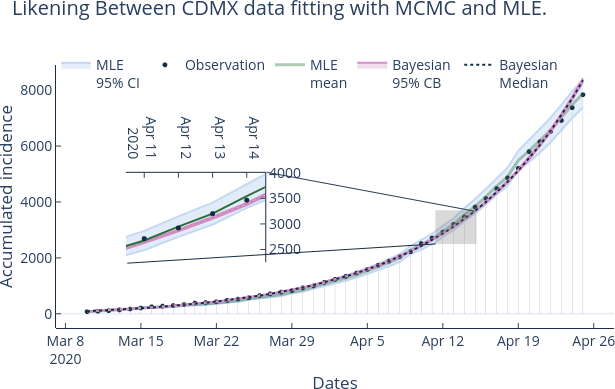
\includegraphics[width=\linewidth]{sto_mle_covid19/Figures/Likening.png}
\end{frame}

        \section{Final comments}
            \begin{frame}{Towards Optimal Stochastic Control of Epidemics}
    \begin{Huge}
        \begin{itemize}
            \item Discrete time
            \item Closed Loop Policies
            \item Games
        \end{itemize}
    \end{Huge}
    \href{https://github.com/SaulDiazInfante/Beamer-xxxii-semana-unison-2022-AppliedMathWorkshop.git}{Git-Hub}
    \\
    \qrcode{https://github.com/SaulDiazInfante/Beamer-xxxii-semana-unison-2022-AppliedMathWorkshop.git}
\end{frame}
 %---------------------------------------------------------------------------
%    \begin{frame}[allowframebreaks]
%        \frametitle{Final Remarks}
%            
%        % \bibliographystyle{acm}
%        \bibliography{main.bib}
%    \end{frame}
\end{document}
